\documentclass{scrartcl}
\usepackage[utf8]{inputenc}
\usepackage[ngerman]{babel}
\usepackage{amsmath}
\usepackage{amssymb}
\usepackage{graphicx}
\usepackage{pdfpages}
\usepackage{color}
\usepackage{booktabs}

\begin{document}
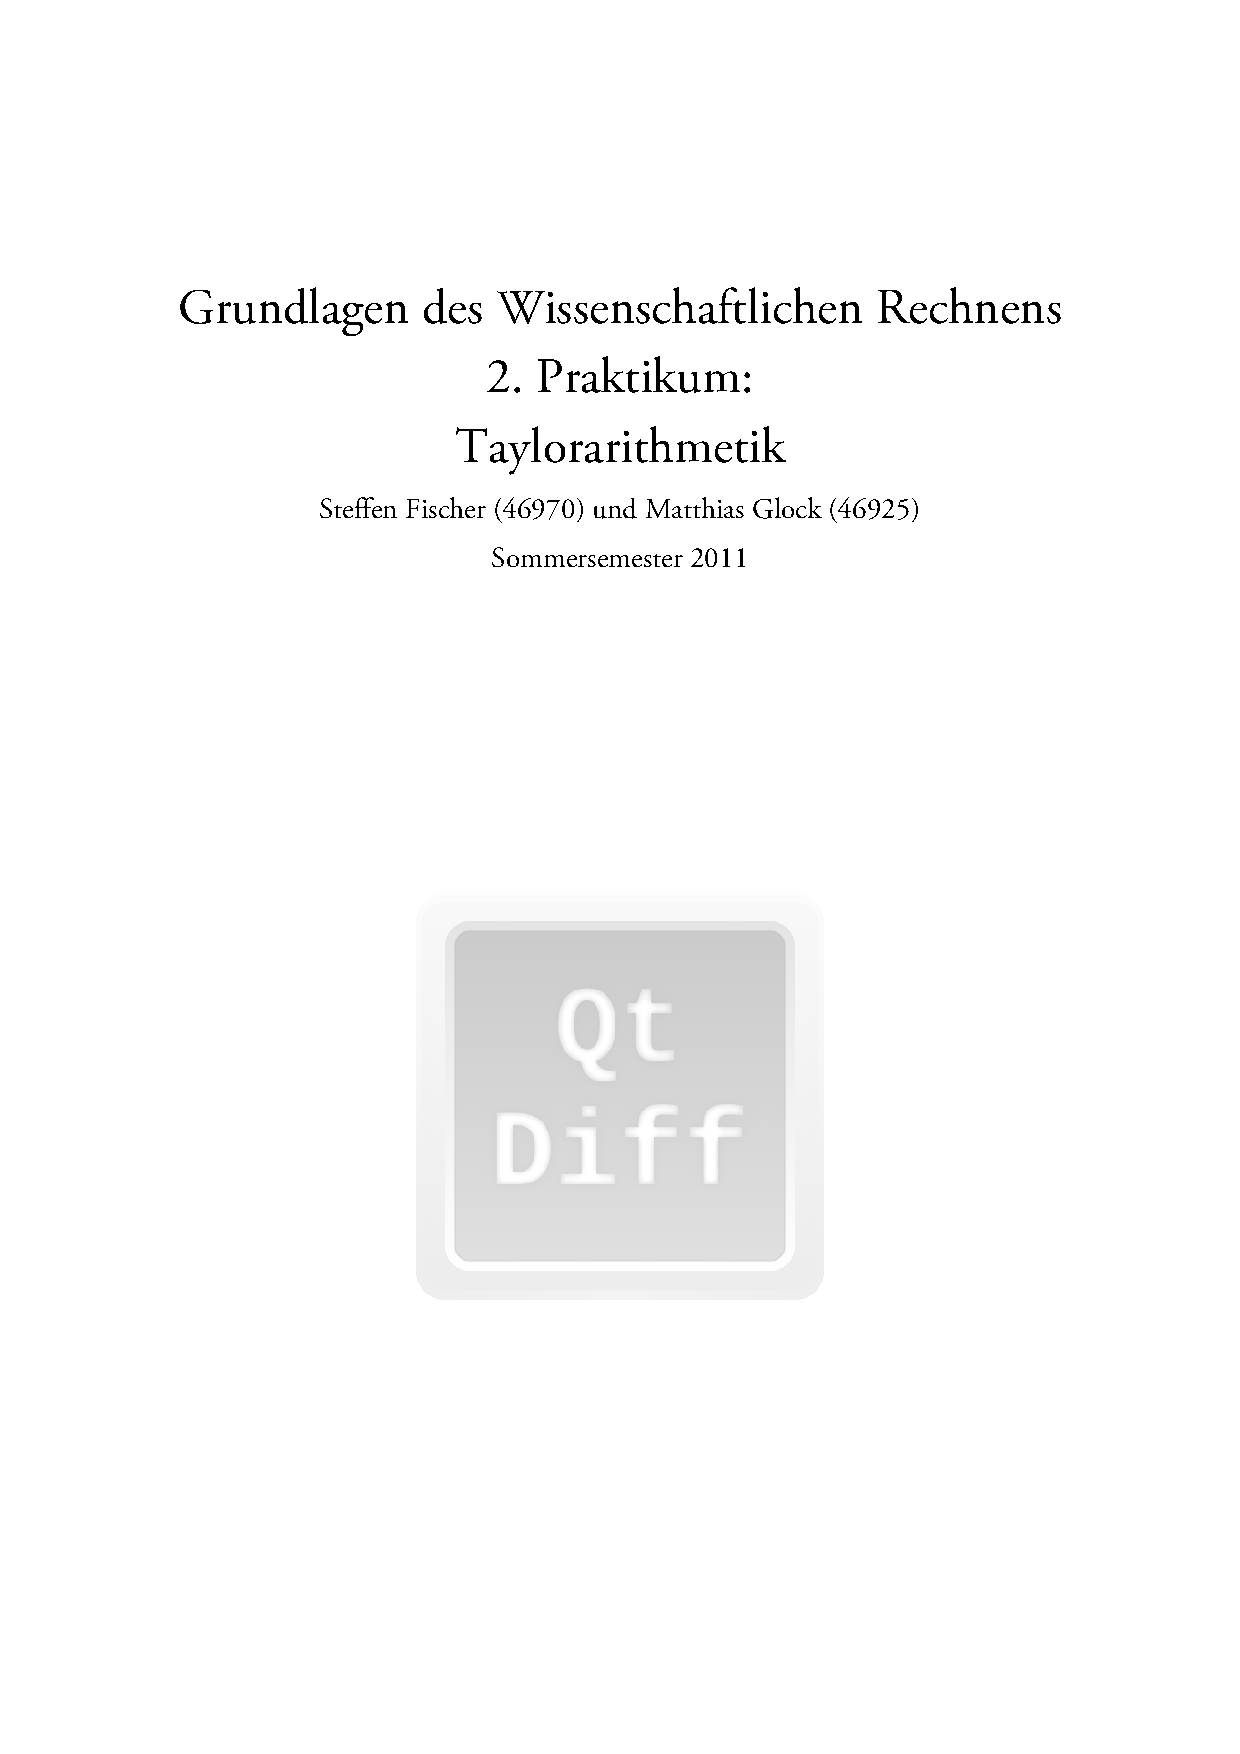
\includepdf{Deckblatt.pdf}
\thispagestyle{empty}
\tableofcontents
\\
\newpage
\setcounter{page}{1}
\section{Aufgabenstellung}
Entwickeln Sie in C++ eine Klasse \textit{Taylor}, die mittels automatischer Differentiation die ersten $n$ Taylorkoeffizienten einer vorgegebenen Funktion berechnet.\\
Implementieren Sie die Grundlagen der Taylorarithmetik und wenden Sie diese auf reelle und tranzendente Funktionen an.\\
Es sind geeignete Konstruktoren (Standardkonstruktor, Kopierkonstruktor, ...) und Destruktoren bereitzustellen.\\
Überladen Sie Operatoren $+,-,*,/$, den Zuweisungsoperator = (wobei die Zuweisung einer Konstanten möglich sein soll), die Ein- und Ausgabeoperatoren sowie mathema-tische Standardfunktionen.\\
Entwickeln Sie ein Demonstrationsprogramm mit einer einfachen Menüsteuerung, welches die Anwendung der Klasse \textit{Taylor} anhand selbstgewählter Beispiele zeigt.

\section{Theoretische Grundlagen}
\subsection{Die Taylorarithmetik}
Grundlage der Taylorarithmetik ist eine Arithmetik von Tupeln
$$(a)_0,(a)_1,...,(a)_k, \ \  (a)_k \in \mathbb{R}$$
Dabei entspricht $(a)_k$ dem $k$-ten Taylorkoeffizienten an der Stelle $t=t_0$.\\
Für die Näherungslösung von Differentiationsgleichungen etc. sind höhere Ableitungen von $u(t)$ sehr nützlich. Kennt man an einer Stelle $t=t_0$ die Werte: $u(t_0), u'(t_0), ... , u^{(n)}(t_0)$,\\
so kann man mittels \textit{Taylorentwicklung} den Wert $u(t)$ mit $t=t_0+h$ approximieren: \\
$$u(t)\approx u_n(t)=\sum\limits_{k=0}^{n}\frac{1}{k!}u^{k}(t_0)\cdot h^k$$
Def.: Der $k$-te Taylorkoeffizient von $u(t)$ für $t=t_0$ lautet: $(u)_k:=\frac{1}{k!}u^{k}(t_0),\ k=0,1,...$\\
\\
Für die Bildung von $(u)_k$ gelten folgende Regeln:\\
(1) Konstanten: $(c)_0=c, (c)_k = 0$ für $k \geq 1$\\
(2) Variable $t$: $(t)_0=t_0, (t)_1= 1, (t)_k =0$ \\
\hspace*{0.5cm} \underline{Beweis:} $\frac{dc}{dt}=0, \frac{dt}{dt}=1, \frac{d^2t}{dt^2}=0$ usw. \\
\\
(3) Arithmetische Regeln: Für $k=1,2,3,...$ gilt :\\
	(3.1) $(u\pm v)_k = (u)_k \pm (v)_k$ \\
	(3.2) $(u \cdot v)_k = \sum_{j=0}^k (u)_k \cdot (v)_{k-j} = \sum_{j=0}^k (u)_{k-j}\cdot(v)_j$\\
	(3.3) $(u/v)_k = \frac{1}{v}\{(u)_k - \sum_{j=1}^k (v)_j \cdot (u/v)_{k-j}$\\
\hspace*{0.5cm}\underline{Beweis:} Mit $h:= t-t_0$ gilt für Funktionen $u,v,w \in \mathbb{C}^{\infty}(\mathbb{R})$ \\
\hspace*{0.5cm}Sei $u(t)= \sum\limits_{k=0}^{\infty} (u)_k \cdot h^k$, $v(t)= \sum\limits_{k=0}^{\infty} (v)_k \cdot h^k$, $w(t)= \sum\limits_{k=0}^{\infty} (w)_k \cdot h^k$ \\
\\
\hspace*{0.5cm}(3.1) $w(t)= u(t)\pm v(t)$\\
	\begin{eqnarray*}\sum_{k=0}^{\infty} (w)_k \cdot h^k &=& \sum_{k=0}^{\infty} (u)_k \cdot h^k \pm \sum_{k=0}^{\infty} (v)_k \cdot h^k\\
 	&=& \sum_{k=0}^{\infty} \left[(u)_k \pm (v)_k\right] \cdot h^k\end{eqnarray*}
\hspace*{0.5cm}durch Koeffizientenvergleich folgt Beh. (3.1)\\
\\
\hspace*{0.5cm}(3.2) $w(t)= u(t)\cdot v(t)$\\ 
	\begin{eqnarray*}\sum_{k=0}^{\infty} (w)_k \cdot h^k &=& \left(\sum_{k=0}^{\infty} (u)_k \cdot h^k \right)\left( \sum_{k=0}^{\infty} (v)_k \cdot h^k\right)\\
 	&=&  \sum_{k=0}^{\infty} \sum_{j=0}^k (u)_j \cdot h^j \cdot (v)_{k-j} \cdot h^{k-j} \\
 	&=& \sum_{k=0}^{\infty} \left(\sum_{j=0}^k (u)_j \cdot (v)_{k-j}\right) \cdot h^{k}\end{eqnarray*}
\hspace*{0.5cm}mit Cauchy-Produkt folgt $(w)_k = \sum\limits_{j=0}^k (u)_j \cdot (v)_{k-j}$ \\
\\
\hspace*{0.5cm}(3.3) Sei $w= u/v$, dann $u = v \cdot w$ mit (3.2) ergibt sich dann:\\
	\begin{eqnarray*}(u)_k &=& \sum_{j=0}^k (v)_j \cdot (w)_{k-j}\\
	 &=& (v)_0 \cdot (w)_k + \sum_{j=1}^k (v)_j \cdot (w)_{k-j}\end{eqnarray*}
\hspace*{0.5cm}umgestellt nach $(w)_k$ folgt $(w)_k = \left((u)_k - \sum\limits_{j=1}^k(v)_j \cdot (w)_{k-j}\right)/v$ und daraus (3.3)
\begin{flushright}$\Box$\end{flushright}\\
\\
Mit den obigen Grundregeln können bereits für die meisten einfachen Funktionen die Taylorkoeffizienten berechnet werden.\\

\newpage
\subsection{Transzendente Funktionen}
Die Taylor-Klasse sollte nun auch noch mit transzendenten Funktionen umgehen können, dazu benötigen wir noch Zusatzregeln, die wie folgt definiert sind:\\
\textit{Hilfsbeziehung} (H): für $k=0,1, ...$ folgt \\
$(u)_{k+1} = \frac{1}{k +1}(u')_k$ bzw. $(u')_k = (k+1)(u)_{k+1}$ \\
\hspace*{0.5cm}\underline{Beweis:} $(u)_{k+1}=\frac{1}{(k+1)!}u^{(k+1)}(t_0) = \frac{1}{k+1}\cdot \frac{1}{k!}\cdot [u'(t)]^{(k)}\Big{|}_{t=t_0} = \frac{1}{k+1}(u')_k $\\
\\
$w = f(u)$ eine transzendente Funktion mit  1.Ableitung $g(u) = f'(u)$\\
\textit{Kettenregel} (K): $w(t) = f(u(t))$ : $w'(t) = f'(u(t)) \cdot u'(t) = g(u(t)) \cdot u'(t)$\\
Falls $g(u)$ differenzierbar, kann man damit $(w)_k$ bestimmen:\\
\begin{align*}k\cdot (w)_k &= (w')_{k-1} \hspace*{4.9cm}\text{nach H}\\
 &= (g(u)\cdot u')_{k-1}\hspace*{4cm}\text{nach K}\\
 &= \sum_{j=0}^{k-1}(g(u))_j\cdot (u')_{k-1-j}\hspace*{2.65cm}\text{nach der Multiplikationsregel}\\
 &= \sum_{j=0}^{k-1} (g(u))_j\cdot (k-j)(u)_{k-j}\hspace*{2cm}\text{nach H}\end{align*}
\begin{equation}\tag{1.}(w)_k = \sum_{j=0}^{k-1} (1-\frac{j}{k})(g(u))_j\cdot (u)_{k-j}\end{equation}\\
Analog ergibt sich aufgrund der Symmetrie der Multiplikationsregel: \\
\begin{equation}\tag{2.}(w)_k = \frac{1}{k}\sum_{j=0}^{k-1} (j+1)\cdot(g(u))_{k-j-1}\cdot (u)_{j+1}\end{equation} \\
\\
Für die transzendenten Funktionen $\exp(u), \sin(u), \cos(u)$ und Potenzfunktion $(u^a)$ nutzt man nun die Zusatzregeln $(1.),(2.)$:
\begin{flushleft}$(\exp(u))_k = \sum_{j=0}^{k-1}(1-\frac{j}{k})\cdot(w)_j \cdot(u)_{k-j}, \ (w)_0 = e^{(u)_0}$\end{flushleft}
\begin{flushleft}$(\sin(u))_k = (w)_k = \frac{1}{k}\sum_{j=0}^{k-1} (j+1)\cdot(\cos(u))_{k-j-1}\cdot (u)_{j+1}$\end{flushleft}
\begin{flushleft}$(\cos(u))_k = (w)_k = -\frac{1}{k}\sum_{j=0}^{k-1} (j+1)\cdot(\sin(u))_{k-j-1}\cdot (u)_{j+1}$\end{flushleft}
\begin{flushleft}$(u^a)_k = \frac{1}{ku} \sum_{j=0}^{k-1}[a\cdot(k-j)-j]\cdot (u)_{k-j} \cdot (u^a)_j, \ a \in \mathbb{R},\ const$\end{flushleft}
\\
\newpage
\noindent Für den Logarithmus $(\ln{u})$ muss speziell eine eigene Herleitung gemacht werden, da $(\frac{1}{u})_j$  nicht zur Verfügung steht, sind die Formeln (1.),(2.) nicht geeignet.\\
Sei $w'=\frac{u'}{u}$\\
\begin{align*}k\cdot(w)_k &= (w')_{k-1}=(\frac{u'}{u})_{k-1}\hspace*{5.75cm}\text{nach H}\\
&= \frac{1}{u}\left\{(u')_{k-1}-\sum_{j=1}^{k-1}(u)_j \cdot (w')_{k-1-j}\right\}\hspace*{2.95cm}\text{nach Quotientenregel}\\  
&= \frac{1}{u}\left\{k\cdot (u)_{k}-\sum_{j=1}^{k-1}(u)_j \cdot (k-j) \cdot (w)_{k-j}\right\}\hspace*{2cm}\text{nach H}\end{align*}\\ 
$$(w)_k=\frac{1}{u}\left\{(u)_{k}-\sum_{j=1}^{k-1} (1-\frac{j}{k})\cdot  (u)_j \cdot (w)_{k-j}\right\}$$\\
\\
\\
Zusätzlich zu diesen transzendenten Funktionen haben wir noch weitere in unserem Programm hinzugefügt, sie werdem wie folgt definiert:
\begin{flushleft}$\tan(x)=\frac{\sin(x)}{\cos(x)}$\end{flushleft}
\begin{flushleft}$\cot(x)=\frac{\cos{x}}{\sin(x)}$\end{flushleft}
\begin{flushleft}$\sinh(x)=\frac{1}{2}\cdot (e^x-e^{-x})$\end{flushleft}
\begin{flushleft}$\cosh(x)=\frac{1}{2}\cdot (e^x+e^{-x})$\end{flushleft}
\begin{flushleft}$\tanh(x)=\frac{\sinh(x)}{\cosh(x)}$\end{flushleft}
\begin{flushleft}$\coth(x)=\frac{\cosh(x)}{\sinh(x)}$\end{flushleft}\\
Für sie sind keine weiteren besonderen Regeln nötig, da sie aus den bereits definierten transzendenten Funktionen zusammengesetzt werden können. 

\newpage
\section{Programmstruktur und Nutzungshinweise}

	\subsection{Grundstruktur}
Als Grundstruktur des Programms dient die grafische Oberfläche (GUI), die im Punkt "`Beschreibung der Bedienung des Programms"' noch näher erläutert wird. Einerseits \mbox{dient} sie dazu, die Dateneingabe zu ermöglichen und andererseits ist sie zuständig für die Ausgabe der errechneten Ergebnisse.\\
Mit der vom Benutzer gemachten Eingabe wird eine Instanz der Klasse \texttt{parser} erstellt, deren Konstruktor übergibt die Eingabe dann als String und evaluiert den eingegebenen Ausdruck. Dabei wird geprüft, ob die Eingabe einen validen Ausdruck enthält. Wenn dies nicht der Fall ist, wird dies dem Benutzer mitgeteilt und keine Berechnung vorgenommen. Im Falle eines validen Ausdrucks wird aus dem Ausdruck rekursiv ein binärer Baum erstellt. Dabei sind die Trennstellen immer die Operatoren im jeweils vorliegenden Ausdruck. Die Rekursion kommt dadurch zu stande, dass der String an einem Operator getrennt wird, und auf diese beiden Teilstrings wiederum der Parser angewendet wird.\\
Sobald der Parser seine Arbeit beendet hat, steht die Instanz von \texttt{parser} bereit um für die Berechnungen von \texttt{autodiff} und \texttt{taylor} verwendet zu werden. Dazu wurden in der Klasse \texttt{parser} für \texttt{autodiff} und \texttt{taylor} zwei rekursive Methoden implementiert, welche dann jeweils mit Differentiations- oder Taylorarithmetik, aus dem binären Baum, das gewünschte Ergebnis berechnen.\\
In Abhängigkeit von den ausgewählten Funktionen in der GUI werden die von \texttt{autodiff} und \texttt{taylor} bereitgestellten Funktionen verwendet.\\
In \texttt{main.cpp} wird eine Instanz der Klasse \texttt{gui} erstellt, welche alle Informationen und Funktionalität der grafischen Oberfläche enthält. Dadurch wird diese in das Hauptprogramm eingebunden.\\
In \texttt{gui.cpp} wird das Aussehen und die Funktionalität der grafischen Oberfläche implementiert. Diese ist sehr ausführlich kommentiert und erklärt sich größtenteils selbst.

\subsection{Aufbau der Klasse Taylor}
        
        \subsubsection{taylor.h}
Hier wird der Quellcode ergänzend zu den bereits vorhandenen Kommentaren im Code selbst weiter erläutert.\\
Die Header-Datei "`taylor.h"' enthält die Deklaration der Klasse. Hier wird deklariert, welche Funktionen Freundfunktionen der Klasse sind, welche Datentypen\hspace*{2} diese\hspace*{2} als Eingabe benötigen und welche zurückgegeben werden. Weiterhin werden die Deklarationen für die überladenen Operatoren angegeben. Die öffentlichen Funktionen für die Klasse sind größtenteils Schnittstellenfunktionen, um von außen Daten manipulieren und auslesen zu können.\\
\newpage
\noindent Listing von "`taylor.h"':
\begin{verbatim}
#ifndef TAYLOR_H
#define TAYLOR_H

#include <math.h>

using namespace std;

class taylor{
        private:
                /**
                 * Anzahl der Taylorkoeefizienten
                 */
                int k;

                /**
                 * Zeiger auf das Array der Taylorkoeefizienten
                 */
                double *ak;
                
        public:
                /**
                 * Konstruktoren
                 */
                taylor();
                taylor(int);
                taylor(int, double *);
                /**
                 * Konstruktor der eine Taylor-Instanz für eine Konstante
                 * oder eine Variable erstellt
                 */
                taylor(char, double, int);
                
                /**
                 * Kopier-Konstruktor, Zuweisungsoperatoren und Destruktor
                 */
                ~taylor();
                taylor &operator =(const taylor &s);
                taylor &operator =(double);
                taylor(const taylor &a);
                
                /**
                 * Methoden zur ausgabe des Koeffizientenarrays, zum setzen der
                 * Taylorkoeffizienten für Konstanten und Variablen
                 * und Berechnung des Wertes des Taylorpolynoms fuer ein festes x
                 */
                double* akout();
                void set_xkoef(double, int);
                void set_ckoef(double, int);
                double xval(double, double, int);

                /**
                 * Durch Freundfunktionen ueberladene Operatoren
                 * und mathematische Funktionen
                 */
                friend taylor operator +(taylor, taylor);
                friend taylor operator -(taylor, taylor);
                friend taylor operator *(taylor, taylor);
                friend taylor operator /(taylor, taylor);
                friend taylor operator -(taylor);
                friend taylor operator *(double, taylor);
                friend taylor sin(taylor);
                friend taylor cos(taylor);
                friend taylor exp(taylor);
                friend taylor ln(taylor);
                friend taylor tan(taylor);
                friend taylor tanh(taylor);
                friend taylor cosh(taylor);
                friend taylor sinh(taylor);
                friend taylor coth(taylor);
                friend taylor cot(taylor);
                friend taylor pow(taylor, taylor);
};
#endif // TAYLOR_H
\end{verbatim}

\subsubsection{taylor.cpp}
In "`taylor.cpp"' wurden alle in "`taylor.h"' deklarierten Funktionen vollständig implementiert. Bei den befreundeten Funktionen sieht man, wie die obigen arithmetischen Gesetze, zur Bildung der Taylorkoeffizienten, implementiert wurden.\\
Weiterhin werden die abgeleiteten transzendenten Funktionen wie beispielsweise $\sinh(x),$ $\cosh(x),$ $\tan(x),$ $\cot(x),$ $\tanh(x)$ und $\coth(x)$ aus den bereits überladenen Funktionen zusammengesetzt.\\
Die von uns auch überladene \texttt{pow(x,y)} Funktion sollte mit Vorsicht verwendet werden, da einerseits die Ableitungen meist falsch sind und sie sich in Grenzfällen auch nicht korrekt verhält. Um Potenzen zu behandeln sollte auf $\exp(x)$ und $\ln(x)$ zurückgegriffen werden.
\newpage
\noindent Listing von "`taylor.cpp"':
\begin{verbatim}
#include "taylor.h"

using namespace std;

/**
 * Default-konstruktor
 */
taylor::taylor(){
        k = 0;
        ak = 0;
}

/**
 * Konstruktor erstellt Instanz mit j Taylorkoeffizienten
 */
taylor::taylor(int j){
        k = j;
        ak = new double[k];
}

/**
 * Konstruktor erstellt Instanz mit j Taylorkoeffizienten
 * und gegebenem Koeffizientenarray
 */
taylor::taylor(int j, double *koeff){
        k = j;
        ak = new double[j];
        ak = koeff;
}

/**
 * Konstruktor erstellt für m gleich 'c' ein Koeffizientenarray der Länge j
 * für eine Konstante mit Wert w oder für m gleich 'x' ein Koeffizientenarray
 * der Länge j für eine Variable mit Wert w
 */
taylor::taylor(char m, double w, int j){
        if(m=='c'){
                k = j;
                ak = new double[k];
                ak[0] = w;
                if(k > 0){
                        for(int i = 1; i < k; i++){
                                ak[i] = 0;
                        }
                }
        }
        else if(m=='x'){
                k = j;
                ak = new double[k];
                ak[0] = w;
                if(k > 0){
                        ak[1] = 1.0;
                        if(k > 1){
                                for(int i = 2; i < k; i++){
                                       ak[i] = 0;
                                }
                        }
                }
        }
        else{
        k = 0;
        ak = 0;
        }
}

/**
 * Schnittstellenfunktionen
 * 
 * set_xkoef() udn set_ckoef() setzten, aehnlich wie obiger Konstruktor,
 * das Koeffizientenarray auf das einer Konstanten bzw. Variablen
 */

void taylor::set_xkoef(double w, int j){
        k = j;
        ak = new double[k];

        ak[0] = w;
        if(k > 0){
                ak[1] = 1.0;
                if(k > 1){
                        for(int i = 2; i < k; i++){
                                ak[i] = 0;
                        }
                }
        }
}

void taylor::set_ckoef(double w, int j){
        k = j;
        ak = new double[k];
        ak[0] = w;
        if(k > 0){			
                for(int i = 1; i < k; i++){
                        ak[i] = 0;
                }
        }
}

/**
 * akout() gibt einen Zeiger auf das Koeffizientenarray zurueck
 */
double* taylor::akout(){
        return ak;
}

double taylor::xval(double x, double t0, int k){
        double x0 = x - t0, tval = ak[k];
        for(int i = k-1; i >= 0; i--){
                tval *= x0;
                tval += ak[i];
        }
        return tval;
}

/**
 * Kopier-Konstruktor, Zuweisungsoperatoren und Destruktor
 */

taylor::taylor(const taylor &a){    
        k = a.k;
        ak = new double[k];
        if( k > 0){
                for(int i = 0; i < k; i++){
                        ak[i] = a.ak[i];
                }
        }
}

taylor &taylor::operator =(const taylor &a){
        k = a.k;
        ak = new double[k];
        if( k > 0){
                for(int i = 0; i < k; i++){
                        ak[i] = a.ak[i];
                }
        }
        else{
                ak = 0;
        }
        return *this;
}

/**
 * = operator kann wie obiger Konstruktor bzw. Methoden
 * das Koeffizientenarray auf das einer Konstanten setzen
 */
taylor &taylor::operator =(double w){
        if(k > 0){
                ak[0] = w;
                if(k > 0){
                        for(int i = 1; i < k; i++){
                                ak[i] = 0;
                        }
                }
        return *this;
        }
}

taylor::~taylor(){
        if(ak != 0) delete[] ak;
}

/**
 * Freundfunktionen fuer ueberladene Operatoren und mathematische Funktionen
 */
taylor operator + (taylor a, taylor b){
        taylor res;
        res.k = a.k;
        res.ak = new double[res.k];
        for(int i = 0; i < res.k; i++){
                res.ak[i] = a.ak[i] + b.ak[i];
        }
        return res;
}
/**
 * unäres Minus
 */
taylor operator -(taylor a){
        taylor res;
        res.k = a.k;
        res.ak = new double[res.k];
        for(int i = 0; i < res.k; i++){
                res.ak[i] = -a.ak[i];
        }
        return res;
}

taylor operator - (taylor a, taylor b){
        taylor res;
        res.k = a.k;
        res.ak = new double[res.k];
        for(int i = 0; i < res.k; i++){
                res.ak[i] = a.ak[i] - b.ak[i];
        }
        return res;
}

taylor operator * (taylor a, taylor b){
        taylor res;
        res.k = a.k;
        res.ak = new double[res.k];
        for(int i = 0; i < res.k; i++){
                res.ak[i]=0;
                for(int j = 0; j <= i; j++){
                        res.ak[i] += (a.ak[i-j] * b.ak[j]);
                }
        }
        return res;
}

taylor operator / (taylor a, taylor b){
        taylor res;
        res.k = a.k;
        res.ak = new double[res.k];
        for(int i = 0; i < res.k; i++){
                res.ak[i] = a.ak[i];
                for(int j = 1; j <= i; j++){
                        res.ak[i] -= (b.ak[j] * res.ak[i-j]);
                }
                res.ak[i] /= b.ak[0];
        }
        return res;
}

/**
 * Sinus und Cosinus werden jeweils parallel berechnet
 */
taylor sin(taylor a){
        taylor sico[2];
        sico[0].k=a.k;
        sico[1].k=a.k;
        sico[0].ak = new double[sico[0].k];
        sico[1].ak = new double[sico[1].k];
	
        sico[0].ak[0] = sin(a.ak[0]);
        sico[1].ak[0] = cos(a.ak[0]);
	
        for(int k = 1; k < a.k; k++){
		
                sico[0].ak[k] = 0;
                sico[1].ak[k] = 0;
		
                for(int j = 0; j < k; j++){
                        sico[0].ak[k] += (j+1) * sico[1].ak[k-j-1] * a.ak[j+1];
                        sico[1].ak[k] += (j+1) * sico[0].ak[k-j-1] * a.ak[j+1];
                }
		
                sico[0].ak[k] /= k;
                sico[1].ak[k] /= -k;
        }
	
        return sico[0];
}

taylor cos(taylor a){
        taylor sico[2];
        sico[0].k=a.k;
        sico[1].k=a.k;
        sico[0].ak = new double[sico[0].k];
        sico[1].ak = new double[sico[1].k];
	
        sico[0].ak[0] = sin(a.ak[0]);
        sico[1].ak[0] = cos(a.ak[0]);
	
        for(int k = 1; k < a.k; k++){
		
                sico[0].ak[k] = 0;
                sico[1].ak[k] = 0;
		
                for(int j = 0; j < k; j++){
                        sico[0].ak[k] += (j+1) * sico[1].ak[k-j-1] * a.ak[j+1];
                        sico[1].ak[k] += (j+1) * sico[0].ak[k-j-1] * a.ak[j+1];
                }
		
                sico[0].ak[k] /= k;
                sico[1].ak[k] /= -k;
        }
	
        return sico[1];
}

taylor exp(taylor a){
        taylor res;
        res.k = a.k;
        res.ak = new double[res.k];
        res.ak[0] = exp(a.ak[0]);
        for(int k = 1; k < res.k; k++){
                res.ak[k] = 0;
                for(int j = 0; j < k; j++){
                        res.ak[k] += (k-j) * res.ak[j] * a.ak[k-j];
                }
                res.ak[k] /= k;
        }
        return res;
}

taylor ln(taylor a){
        taylor res;
        res.k = a.k;
        res.ak = new double[res.k];
        res.ak[0] = log(a.ak[0]);
        for(int k = 1; k < res.k; k++){
                res.ak[k] = a.ak[k];
                for(int j = 1; j < k; j++){
                        res.ak[k] -= (1-double(j)/double(k)) * a.ak[j] * res.ak[k-j];
                }
                res.ak[k] /= a.ak[0];
        } 
        return res;
}

/**
 * tan(), cosh(), sinh(), tanh(), cot() und coth() koennen nun
 * mithilfe obiger Funktionen definiert werden
 */
taylor tan(taylor a){
        return sin(a)/cos(a);
}

taylor cosh(taylor a){
        taylor c('c',0.5,a.k);
        return c*(exp(a)+exp(-a));
}

taylor sinh(taylor a){
        taylor c('c',0.5,a.k);
        return c*(exp(a)-exp(-a));
}

taylor tanh(taylor a){
        return sinh(a)/cosh(a);
}

taylor cot(taylor a){
        return cos(a)/sin(a);
}

taylor coth(taylor a){
        return cosh(a)/sinh(a);
}

/**
 * pow() fungiert als fast funktionierede Potenzfunktion
 */
taylor pow(taylor u, taylor v){	
        taylor res;
        res.k = u.k;
        res.ak = new double[res.k];
        if (u.ak[0] == 0){
                res.set_ckoef(0, res.k);
                return res;
        }
        else if (v.ak[0] == 0){
                res.set_ckoef(1, res.k);
                return res;
        }
        else if (u.ak[0] == exp(1)){
                return exp(v);
        }
        else if(int(v.ak[0]*10.0) == int(v.ak[0])*10 && v.ak[1] == 0)
        {	
                res = u;
		
                for(int i = 0; i < int(v.ak[0])-1; i++){
                        res = res * u;
                }
                return res;
        }
        else
        {
                if(u.ak[0] < 0){
                        return exp(v * ln(-u));
                }
                else{
                        return exp(v * ln(u));
                }
        }
}
\end{verbatim}
\newpage
\subsubsection{parser.cpp}

Um den vom Parser erstellten binären Baum auszuwerten, haben wir eine rekursive Funktion geschrieben, welche den Baum durchläuft und dabei immer die an einem Knoten stehenden Operationen auf die beiden Äste des Knotens anwendet. Hierbei ist die Abbruchbedingung, dass wir bei einem Blatt angelangt sind, was man daran erkennt, dass ein Knoten keine Äste mehr besitzt.\\
In der \texttt{switch}-Verzweigung sieht man sehr gut, wie die überladenen Operatoren rekursiv angewendet werden. Durch den zweifachen Aufruf von \texttt{parser::tayl} in vielen Rekursionsschritten liegt hier eine nicht-lineare Rekursion vor.\\
\\
Auszug aus "`parser.cpp"':
\begin{verbatim}
taylor parser::tayl(int k,double x, Baum term){
        if ((term.l == 0)&&(term.r == 0)){	
		
                // Instanz von taylor einer Variable mit Wert x wird erstellt
                if(term.text == "x"){
                        taylor tx('x',x,k);
                        return tx;
                }
		
                // Konstante e wird korrekt erkannt
                if(term.text == "e"){
                        taylor tc('c',exp(1),k);
                        return tc;
                }
		
                // ansonsten wird Instanz einer Konstanten mit dem Wert in term.text
                // (welcher mit atof(..) in double umgewandelt wurde) zurückgegeben
                taylor tc('c', atof(term.text.c_str()), k);
                return tc;		
        }
        else{
                switch(term.op){
                // Je nach Operator werden die benötigten für taylor überladenen
                // Freundfunktionen angewendet.
                        case 2:
                                return pow(tayl(k,x,*term.l), tayl(k,x,*term.r));
                        case 3:				
                                return tayl(k,x,*term.l)*tayl(k,x,*term.r);
                        case 4:				
                                return tayl(k,x,*term.l)/tayl(k,x,*term.r);
                        case 5:				
                                return tayl(k,x,*term.l)-tayl(k,x,*term.r);
                        case 6:		
                                return tayl(k,x,*term.l)+tayl(k,x,*term.r);
                        case 20:						
                                return exp(tayl(k,x,*term.r));
                        case 21:						
                                return sin(tayl(k,x,*term.r));
                        case 22:						
                                return cos(tayl(k,x,*term.r));
                        case 23:						
                                return ln(tayl(k,x,*term.r));
                        case 24:						
                                return tan(tayl(k,x,*term.r));
                        case 25:						
                                return sinh(tayl(k,x,*term.r));
                        case 26:						
                                return cosh(tayl(k,x,*term.r));
                        case 27:						
                                return tanh(tayl(k,x,*term.r));
                        case 28:						
                                return cot(tayl(k,x,*term.r));
                        case 29:						
                                return coth(tayl(k,x,*term.r));
                }		
        }
}
\end{verbatim}

\subsection{Beschreibung der Bedienung des Programms}
		
Für die Bedienung des Programms haben wir uns entschieden eine graphische Oberfläche zu entwickeln, die im Gegensatz zu einer Menüsteuerung innerhalb der Konsole wesentlich benutzerfreundlicher ist. Zum Bauen der Oberfläche haben wir den QT-Designer benutzt, der uns die Möglichkeit gibt das Fenster des Programms nach belieben zu gestalten. Wir haben das Fenster so gestaltet, dass der Benutzer seine Eingabe einfach in das Eingabefeld schreibt und ihm die Möglichkeit gegeben zwischen den einzelnen Funktionen unseres Programms auszuwählen. Diese werden mittels Checkboxen ein- bzw. ausgeschaltet. Zunächst kann man zwischen den beiden Differentiationsklassen Autodiff und Taylor auswählen. \\
Nun kann man in Autodiff zwischen drei verschiedenen Ausgaben wählen. Zum einen gibt es die Möglichkeit an einem bestimmten selbstwählbaren Punkt den Funktionswert, sowie die Werte der ersten und zweiten Ableitung, ausgeben zu lassen. Desweiteren kann man beim Unterpunkt Newton eine Newton-Iteration ausführen lassen bei der man sich so über den Startwert $s$ und die Genauigkeit $d$ die Nullstelle annähern lässt. \mbox{Zuletzt} haben wir die Auswahl einer Wertetabelle zur Verfügung gestellt, über die sich der Nutzer, in einem selbstgewählten Intervall mit bestimmbar großen Zwischenschritten, Werte ausgeben lassen kann.\\
Im Unterpunkt Taylor kann man über die Checkboxen den Entwicklungspunkt $t_0$, die Anzahl $k$ der zu berechnenden Taylorkoeffizienten  und den $x$-Wert, an welchem das Taylorpolynom ausgewertet werden soll festlegen. Im Ausgabebereich wird schließlich das Taylorpolynom bis zum k-ten Glied und dessen Wert an der Stelle $x$ ausgegeben.\\
Außerdem haben wir noch eine Funktion "`Plot"' hinzugefügt. Über diese Checkbox hat man die Möglichkeit, unabhängig von den Klassen Autodiff und Taylor, die Eingabe in einem selbstgewählten Intervall plotten zu lassen. Dabei kann man sowohl das x- als auch das y-Achsen-Intervall bestimmen. Zudem kann man die Genauigkeit des Plots bestimmen. Außerdem werden bei der Aktivierung von Autodiff die ersten beiden Ableitungen und bei der Aktivierung von Taylor die ersten $k$ Annäherungen durch Taylorpolynome noch zusätzlich mit in den Plot integriert.\\
Wenn der Nutzer seine gewünschte Funktion eingegeben hat, kann er sich das Ergebnis entweder über den Button "`Calculate"' oder die Eingabetaste ausgeben lassen.\\
Um das Ausgabefeld von den bereits ausgerechneten Ergebnissen zu bereinigen haben wir den Button "`Clear"' eingebaut.\\
Mit dem "`Help"'-Button kann der Benutzer sich Informationen über die Benutzung des Programms holen. Es werden die zulässigen Eingaben erläutert und außerdem zu den einzelnen Funktionen kurze Erklärungen zur Verfügung gestellt.\\ 
\begin{center}
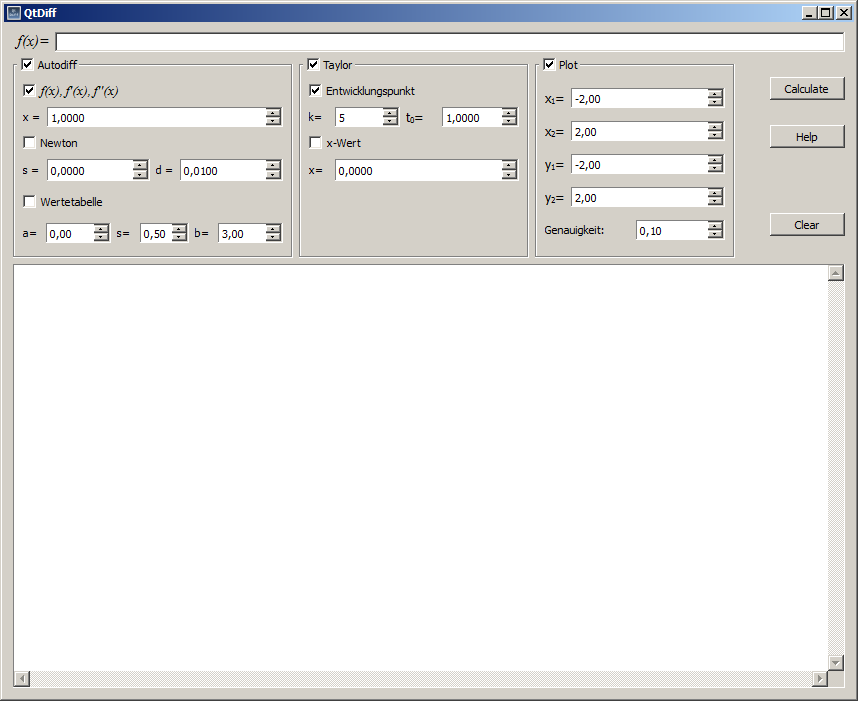
\includegraphics[width=12cm]{./png/Gui1.png}
\\
\footnotesize{Gui-Erscheinungsbild unter Windows 7 - Classic}
\end{center}

\subsection{Nutzungshinweise}
Das Programm bietet mit dem \texttt{\^{ }}-Operator zwar die Funktionalität einen Ausdruck zu potenzieren. Doch dieser funktioniert nicht immer korrekt, weshalb er mit Vorsicht zu benutzen ist.\\
Weiterhin wird beim Plotten in den Unterordner \texttt{/plots} für jeden einzelnen Plot ein Bild erstellt. Diese Bilder erhalten immer ein Suffix in Form einer Zufallszahl. Somit häufen sie sich mit der Zeit in diesem Ordner an und sollten deshalb von Zeit zu Zeit gelöscht werden. Dies bietet aber die Möglichkeit auch sehr einfach Sicherungen von interessanten Plots zu erstellen.

\newpage
\section{Beispiele}
	\subsection{Standartfunktionen}
Zunächst verwenden wir unser Programm um die, von uns implementierten mathematischen Standartfunktionen zu testen. Die Anzahl $k$ der Koeffizienten beträgt 8 und der Entwicklungspunkt $t_0$ ist 0 bzw. 1 bei $\ln$, $\cot$ und $\coth$. Damit ergeben sich für die Funktionen folgende Taylorpolynome $T(x)$.\\
\\
$f(x)=\exp(x)$:
\begin{verbatim}
T(x) = 1 + 1 * x + 0.5 * x^2 + 0.166667 * x^3 + 0.0416667 * x^4 + 0.00833333 * x^5
       + 0.00138889 * x^6 + 0.000198413 * x^7 + R(xi)
\end{verbatim}
$f(x)=\ln(x)$:
\begin{verbatim}
T(x) = 0 + 1 * (x-1) + -0.5 * (x-1)^2 + 0.333333 * (x-1)^3 + -0.25 * (x-1)^4
       + 0.2 * (x-1)^5 + -0.166667 * (x-1)^6 + 0.142857 * (x-1)^7 + R(xi)
\end{verbatim}
$f(x)=\sin(x)$:
\begin{verbatim}
T(x) = 0 + 1 * x + -0.166667 * x^3 + 0.00833333 * x^5 + -0.000198413 * x^7 + R(xi)
\end{verbatim}
$f(x)=\cos(x)$:
\begin{verbatim}
T(x) = 1 + -0.5 * x^2 + 0.0416667 * x^4 + -0.00138889 * x^6 + R(xi)
\end{verbatim}
$f(x)=\tan(x)$:
\begin{verbatim}
T(x) = 0 + 1 * x + 0.333333 * x^3 + 0.133333 * x^5 + 0.0539683 * x^7 + R(xi)
\end{verbatim}
$f(x)=\cot(x)$:
\begin{verbatim}
T(x) = 0.642093 + -1.41228 * (x-1) + 0.906816 * (x-1)^2 + -1.05302 * (x-1)^3
       + 0.978409 * (x-1)^4 + -1.01062 * (x-1)^5 + 0.9952 * (x-1)^6
       + -1.00227 * (x-1)^7 + R(xi)
\end{verbatim}
$f(x)=\sinh(x)$:
\begin{verbatim}
T(x) = 0 + 1 * x + 0.166667 * x^3 + 0.00833333 * x^5 + 0.000198413 * x^7 + R(xi)
\end{verbatim}
$f(x)=\cosh(x)$:
\begin{verbatim}
T(x) = 1 + 0.5 * x^2 + 0.0416667 * x^4 + 0.00138889 * x^6 + R(xi)
\end{verbatim}
$f(x)=\tanh(x)$:
\begin{verbatim}
T(x) = 0 + 1 * x + -0.333333 * x^3 + 0.133333 * x^5 + -0.0539683 * x^7 + R(xi)
\end{verbatim}
$f(x)=\coth(x)$:
\begin{verbatim}
T(x) = 1.31304 + -0.724062 * (x-1) + 0.950719 * (x-1)^2 + -1.00697 * (x-1)^3
       + 1.00528 * (x-1)^4 + -1.00041 * (x-1)^5 + 0.999602 * (x-1)^6
       + -0.999889 * (x-1)^7 + R(xi)
\end{verbatim}
\newpage
\noindent Zur Demonstration unserer Klasse haben wir uns folgende komplexere Funktionen ausgesucht:\\
$f(x)=e^{-x^2}$\\
$f(x)=0.25*x*(x^2-1)*(x^2-4)$\\
$f(x)=e^{(\sin(x)+\cos(x))}$

\subsection{$f(x)=e^{-x^2}$}
Dafür ist folgende Eingabe zu tätigen: $f(x)=$ \texttt{exp(-x\^{ }2)} oder \texttt{f(x)=e\^{ }(-x\^{ }2)}\\
Bei Anzahl der Koeffizienten: $k=5$\\
Bei Entwicklungspunkt: $t_0=1$\\
Bei x-Wert: $x=0$\\
Das Programm liefert dann diese Ausgabe:
\begin{verbatim}
> Input interpretation: f(x) = exp(-x^2)
 
> Taylorpolynom: 

     T(x) = 0.367879 + -0.735759 * (x-1) + 0.367879 * (x-1)^2 + 0.245253 * (x-1)^3
            + -0.306566 * (x-1)^4 + R(xi)

> Wert des Taylerpolynoms bei x=0

     T(0) = 0.919699

> Plot:
\end{verbatim}

\begin{center}
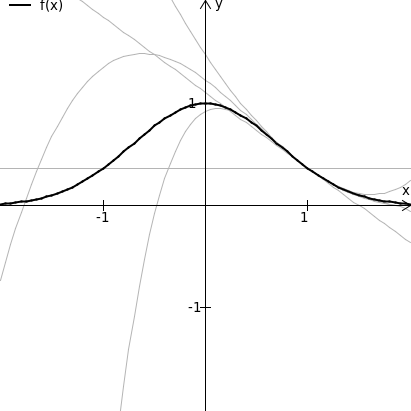
\includegraphics[width=8cm]{./png/plot_gauss.png}
\end{center}

\newpage
	\subsection{$f(x)=0.25\cdot x(x^2-1)(x^2-4)$}
Dafür ist folgende Eingabe zu tätigen: $f(x)=$ \texttt{0.25*x*(x\^{ }2-1)*(x\^{ }2-4)} \\
Bei Anzahl der Koeffizienten: $k=6$\\
Bei Entwicklungspunkt: $t_0=1$\\
Bei x-Wert: $x=2$\\
Das Programm liefert dann diese Ausgabe:
\begin{verbatim}
> Input interpretation: f(x) = 0.25*x*(x^2-1)*(x^2-4)
 
> Taylorpolynom: 

     T(x) = 0 + -1.5 * (x-1) + -1.25 * (x-1)^2 + 1.25 * (x-1)^3 + 1.25 * (x-1)^4
            + 0.25 * (x-1)^5 + R(xi)

> Wert des Taylerpolynoms bei x=2

     T(2) = 0

> Plot:
\end{verbatim}
\begin{center}
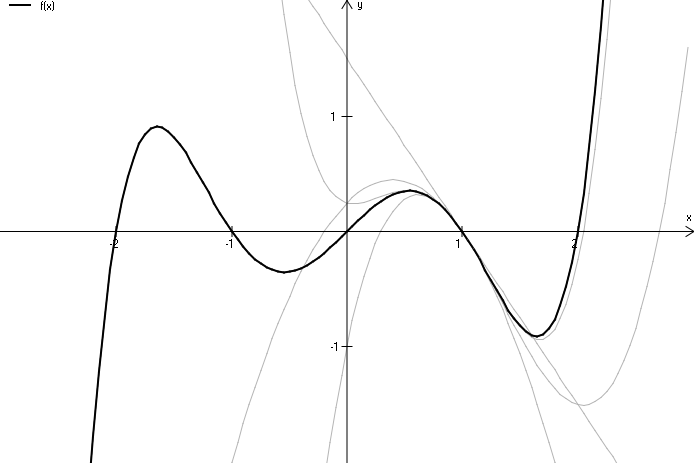
\includegraphics[width=10cm]{./png/plot_ploynom.png}
\end{center}
\newpage
	\subsection{$f(x)=e^{(\sin(x)+\cos(x))}$}
Dafür ist folgende Eingabe zu tätigen: $f(x)=$ \texttt{exp(sin(x)+cos(x))}\\
Bei Anzahl der Koeffizienten: $k=7$\\
Bei Entwicklungspunkt: $t_0=-1$\\
Bei x-Wert: $x=0$\\
Das Programm liefert dann diese Ausgabe:
\begin{verbatim}
> Input interpretation: f(x) = exp(sin(x)+cos(x))
 
> Taylorpolynom: 

     T(x) = 0.739953 + 1.02245 * (x+1) + 0.81782 * (x+1)^2 + 0.308916 * (x+1)^3
            + -0.0175958 * (x+1)^4 + -0.101004 * (x+1)^5 + -0.0564361 * (x+1)^6 + R(xi)

> Wert des Taylerpolynoms bei x=0

     T(0) = 2.7141

> Plot:
\end{verbatim}	
\begin{center}
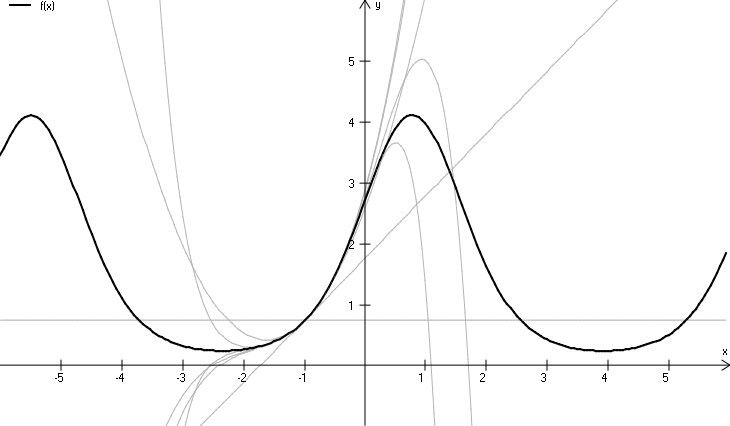
\includegraphics[width=10cm]{./png/plot_expsincos.png}
\end{center}

	\newpage
\section{Literaturhinweise}
	\begin{enumerate}\item \textbf{Fornberg, B.} A Partical Guide to Pseudospectral Methods. University Press, Cambridge, 1996\\
	\item \textbf{Vogt, W.} Vorlesungsskript Techniken des Wissenschaftlichen Rechnens. Abschnitt 3 - Automatisches Differenzieren. \\
	\item \textbf{Lohner, R.} einschließung der Lösung gewöhnlicher Anfangs- und Randwertaufgaben und Anwendungen. Dissertation.(TU-Bibliothek)\\
	\item \textbf{Wolf, J.} Qt 4.6 GUI-Entwicklung mit C++. Galileo Press, Bonn, 2010\\
	\item \textbf{Willemer, A.} Einstieg in C++. Galileo Computing, Bonn, 2007
	\item \textbf{Blomquist F., Hofschuster W., Krämer W.} Real and Complex Taylor Arithmetic in C-XSC, Bergische Universität Wuppertal, 2005
	\end{enumerate}
        \textcolor{white}{bam}
\end{document}
